%%%%%%%%%%%%%%%%%%%%%%%%%%%%%%%%%%%%%%%%%
% Programming/Coding Assignment
% LaTeX Template
%
% This template has been downloaded from:
% http://www.latextemplates.com
%
% Original author:
% Ted Pavlic (http://www.tedpavlic.com)
%
% Note:
% The \lipsum[#] commands throughout this template generate dummy text
% to fill the template out. These commands should all be removed when 
% writing assignment content.
%
% This template uses a Perl script as an example snippet of code, most other
% languages are also usable. Configure them in the "CODE INCLUSION 
% CONFIGURATION" section.
%
%%%%%%%%%%%%%%%%%%%%%%%%%%%%%%%%%%%%%%%%%

%----------------------------------------------------------------------------------------
%	PACKAGES AND OTHER DOCUMENT CONFIGURATIONS
%----------------------------------------------------------------------------------------

\documentclass[a4paper]{article}

\usepackage{fancyhdr} % Required for custom headers
\usepackage{lastpage} % Required to determine the last page for the footer
\usepackage{extramarks} % Required for headers and footers
\usepackage[usenames,dvipsnames]{color} % Required for custom colors
\usepackage{graphicx} % Required to insert images
\usepackage{listings} % Required for insertion of code
\usepackage{courier} % Required for the courier font
\usepackage{lipsum} % Used for inserting dummy 'Lorem ipsum' text into the template
\usepackage{multirow}
\usepackage{tabu}
\usepackage{float}

% Margins
\topmargin=-0.45in
\evensidemargin=0in
\oddsidemargin=0in
\textwidth=6.5in
\textheight=9.5in
\headsep=0.25in

\linespread{1.1} % Line spacing

% Set up the header and footer
\pagestyle{fancy}
\lhead{\hmwkAuthorName} % Top left header
\chead{\hmwkShortTitle} % Top center head
\rhead{\firstxmark} % Top right header
\lfoot{\lastxmark} % Bottom left footer
\cfoot{} % Bottom center footer
\rfoot{Page\ \thepage\ of\ \protect\pageref{LastPage}} % Bottom right footer
\renewcommand\headrulewidth{0.4pt} % Size of the header rule
\renewcommand\footrulewidth{0.4pt} % Size of the footer rule

\setlength\parindent{0pt} % Removes all indentation from paragraphs

%----------------------------------------------------------------------------------------
%	CODE INCLUSION CONFIGURATION
%----------------------------------------------------------------------------------------

\definecolor{MyDarkGreen}{rgb}{0.0,0.4,0.0} % This is the color used for comments
\lstloadlanguages{Matlab} % Load Perl syntax for listings, for a list of other languages supported see: ftp://ftp.tex.ac.uk/tex-archive/macros/latex/contrib/listings/listings.pdf
\lstset{language=Matlab, % Use Perl in this example
        frame=single, % Single frame around code
        basicstyle=\small\ttfamily, % Use small true type font
        keywordstyle=[1]\color{Blue}\bf, % Perl functions bold and blue
        keywordstyle=[2]\color{Purple}, % Perl function arguments purple
        keywordstyle=[3]\color{Blue}\underbar, % Custom functions underlined and blue
        identifierstyle=, % Nothing special about identifiers                                         
        commentstyle=\usefont{T1}{pcr}{m}{sl}\color{MyDarkGreen}\small, % Comments small dark green courier font
        stringstyle=\color{Purple}, % Strings are purple
        showstringspaces=false, % Don't put marks in string spaces
        tabsize=5, % 5 spaces per tab
        %
        % Put standard Perl functions not included in the default language here
        morekeywords={rand},
        %
        % Put Perl function parameters here
        morekeywords=[2]{on, off, interp},
        %
        % Put user defined functions here
        morekeywords=[3]{test},
       	%
        morecomment=[l][\color{Blue}]{...}, % Line continuation (...) like blue comment
        numbers=left, % Line numbers on left
        firstnumber=1, % Line numbers start with line 1
        numberstyle=\tiny\color{Blue}, % Line numbers are blue and small
        stepnumber=5 % Line numbers go in steps of 5
}

% Creates a new command to include a perl script, the first parameter is the filename of the script (without .pl), the second parameter is the caption
\newcommand{\matlabscript}[2]{
\begin{itemize}
\item[]\lstinputlisting[caption=#2,label=#1]{#1.m}
\end{itemize}
}

%----------------------------------------------------------------------------------------
%	DOCUMENT STRUCTURE COMMANDS
%	Skip this unless you know what you're doing
%----------------------------------------------------------------------------------------

% Header and footer for when a page split occurs within a problem environment
\newcommand{\enterProblemHeader}[1]{
\nobreak\extramarks{#1}{#1 continued on next page\ldots}\nobreak
\nobreak\extramarks{#1 (continued)}{#1 continued on next page\ldots}\nobreak
}

% Header and footer for when a page split occurs between problem environments
\newcommand{\exitProblemHeader}[1]{
\nobreak\extramarks{#1 (continued)}{#1 continued on next page\ldots}\nobreak
\nobreak\extramarks{#1}{}\nobreak
}

\setcounter{secnumdepth}{0} % Removes default section numbers
\newcounter{homeworkProblemCounter} % Creates a counter to keep track of the number of problems

\newcommand{\homeworkProblemName}{}
\newenvironment{homeworkProblem}[1][Problem \arabic{homeworkProblemCounter}]{ % Makes a new environment called homeworkProblem which takes 1 argument (custom name) but the default is "Problem #"
\stepcounter{homeworkProblemCounter} % Increase counter for number of problems
\renewcommand{\homeworkProblemName}{#1} % Assign \homeworkProblemName the name of the problem
\section{\homeworkProblemName} % Make a section in the document with the custom problem count
\enterProblemHeader{\homeworkProblemName} % Header and footer within the environment
}{
\exitProblemHeader{\homeworkProblemName} % Header and footer after the environment
}

\newcommand{\problemAnswer}[1]{ % Defines the problem answer command with the content as the only argument
\noindent\framebox[\columnwidth][c]{\begin{minipage}{0.98\columnwidth}#1\end{minipage}} % Makes the box around the problem answer and puts the content inside
}

\newcommand{\homeworkSectionName}{}
\newenvironment{homeworkSection}[1]{ % New environment for sections within homework problems, takes 1 argument - the name of the section
\renewcommand{\homeworkSectionName}{#1} % Assign \homeworkSectionName to the name of the section from the environment argument
\subsection{\homeworkSectionName} % Make a subsection with the custom name of the subsection
\enterProblemHeader{\homeworkProblemName\ [\homeworkSectionName]} % Header and footer within the environment
}{
\enterProblemHeader{\homeworkProblemName} % Header and footer after the environment
}

%----------------------------------------------------------------------------------------
%	NAME AND CLASS SECTION
%----------------------------------------------------------------------------------------

\newcommand{\hmwkTitle}{CO395 Machine Learning\\CBC \#1\\Decision Trees} % Assignment title
\newcommand{\hmwkShortTitle}{CBC \#1 - Decision Trees}
\newcommand{\hmwkDueDate}{Monday,\ November\ 4,\ 2013} % Due date
\newcommand{\hmwkAuthorName}{Group 1} % Your name

%----------------------------------------------------------------------------------------
%	TITLE PAGE
%----------------------------------------------------------------------------------------

\title{
\vspace{2in}
\textmd{\textbf{\hmwkTitle}}\\
%\normalsize\vspace{0.1in}\small{Due\ on\ \hmwkDueDate}\\
%\vspace{0.1in}\large{\textit{\hmwkClassInstructor\ \hmwkClassTime}}
\vspace{3in}
\textbf{Group 1}\\
Yong Wen Chua, \texttt{ywc110}\\
Thomas Morrison, \texttt{tm1810}\\
Marcin Baginski, \texttt{mgb10}\\
Marcin Kadziela, \texttt{mk4910}
}

%\author{\textbf{\hmwkAuthorName}}

\date{} % Insert date here if you want it to appear below your name

%----------------------------------------------------------------------------------------

\begin{document}

\maketitle

%----------------------------------------------------------------------------------------
%	TABLE OF CONTENTS
%----------------------------------------------------------------------------------------

%\setcounter{tocdepth}{1} % Uncomment this line if you don't want subsections listed in the ToC

\newpage
\tableofcontents
\newpage

%----------------------------------------------------------------------------------------
%	EXAMPLES
%----------------------------------------------------------------------------------------

% Example how to paste code into the report:
%
% Listing \ref{LIFDemo} shows a Matlab script.
% \matlabscript{LIFDemo}{Sample Perl Script With Highlighting}

% Example how to paste a figure into the report:
% \begin{figure}
% \center
% 
\includegraphics[width=0.75\columnwidth]{example_figure} % Example image
% \caption{sometext}
% \end{figure}

% Ready code for the confusion matrix:
%
%\begin{table}
%\center
%\begin{tabu}{cc|c|c|c|c|c|c|}
%\cline{3-8}
%& & \multicolumn{6}{ c| }{Predicted class} \\ \cline{3-8}
%& & 1 & 2 & 3 & 4 & 5 & 6 \\ \cline{1-2} \tabucline[1.5pt]{3-8}
%\multicolumn{1}{ |c| }{\multirow{6}{*}{Actual class} } &
%\multicolumn{1}{ |c|[1.5pt] }{1} & 0 & 0 & 0 & 0 & 0 & 0     \\ \cline{2-8}
%\multicolumn{1}{ |c| }{}                        &
%\multicolumn{1}{ |c|[1.5pt] }{2} & 0 & 0 & 0 & 0 & 0 & 0     \\ \cline{2-8}
%\multicolumn{1}{ |c|  }{}                        &
%\multicolumn{1}{ |c|[1.5pt] }{3} & 0 & 0 & 0 & 0 & 0 & 0     \\ \cline{2-8}
%\multicolumn{1}{ |c|  }{}                        &
%\multicolumn{1}{ |c|[1.5pt] }{4} & 0 & 0 & 0 & 0 & 0 & 0     \\ \cline{2-8}
%\multicolumn{1}{ |c|  }{}                        &
%\multicolumn{1}{ |c|[1.5pt] }{5} & 0 & 0 & 0 & 0 & 0 & 0     \\ \cline{2-8}
%\multicolumn{1}{ |c|  }{}                        &
%\multicolumn{1}{ |c|[1.5pt] }{6} & 0 & 0 & 0 & 0 & 0 & 0     \\ \cline{1-8}
%\end{tabu}
%\caption{Confusion Matrix}
%\label{confusionMatrix}
%\end{table}

%----------------------------------------------------------------------------------------
%	SECTION 1 - Implementation Details
%----------------------------------------------------------------------------------------

\section{Implementation Details}

\clearpage

%----------------------------------------------------------------------------------------
%	SECTION 2 - Tree Figures
%----------------------------------------------------------------------------------------

\section{Tree Figures}

\begin{figure}[!ht]
\center
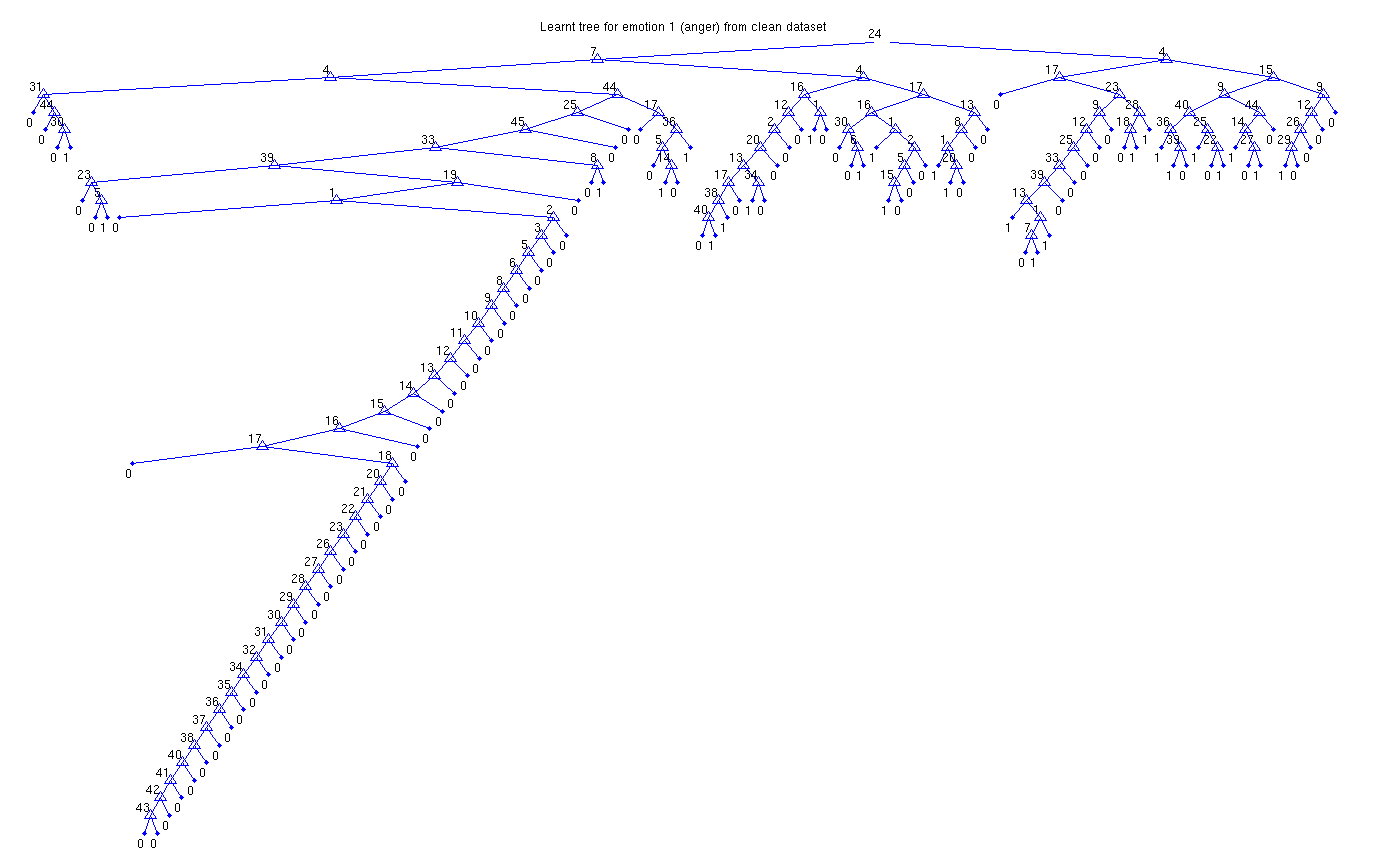
\includegraphics[width=0.75\columnwidth]{AngerTree} % Example image
\caption{Trained decsion tree on the clean dataset for emotion 1 (anger)}
\end{figure}

\bigskip\bigskip\bigskip\bigskip\bigskip\bigskip\bigskip

\begin{figure}[!ht]
\center
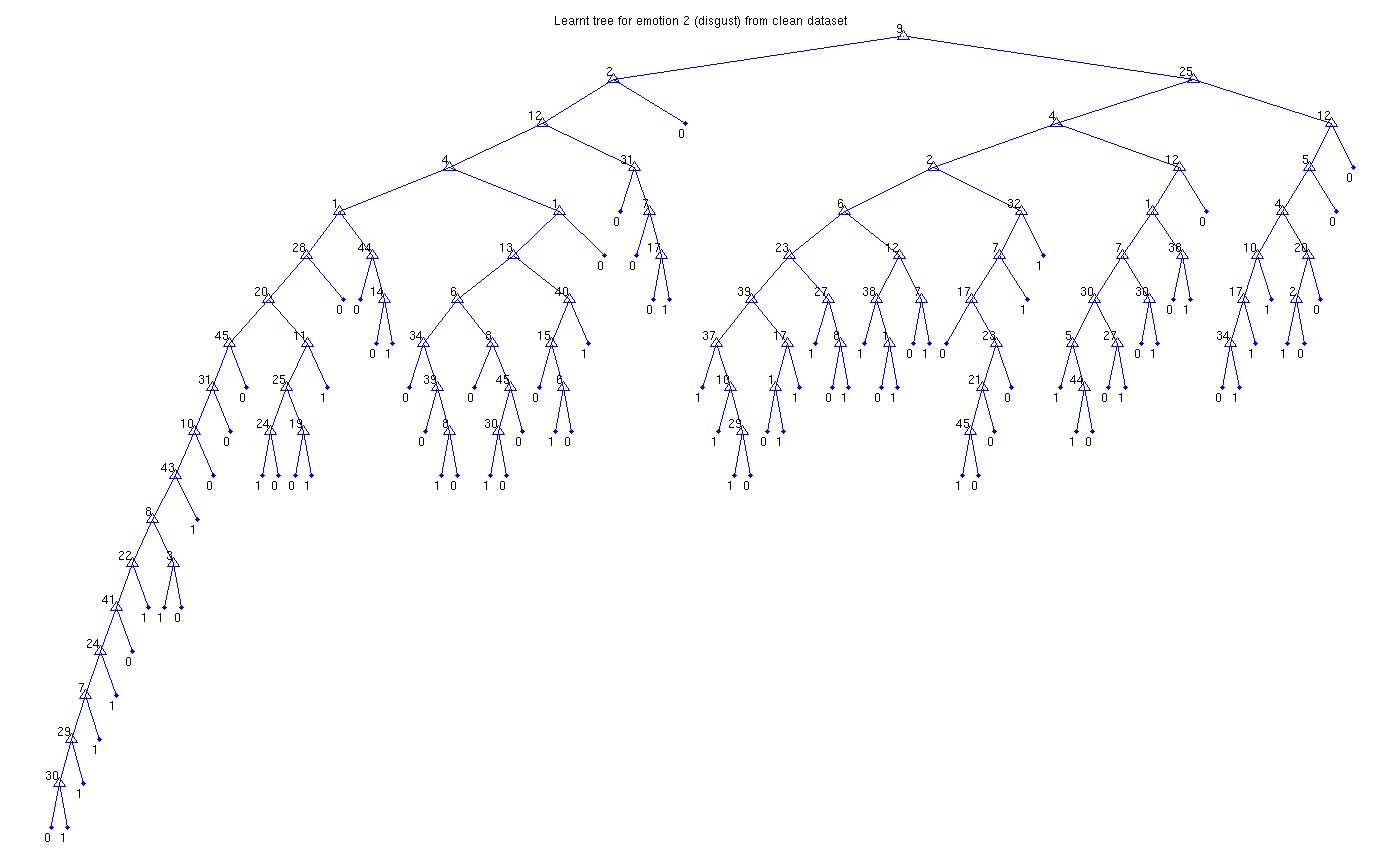
\includegraphics[width=0.75\columnwidth]{DisgustTree} % Example image
\caption{Trained decsion tree on the clean dataset for emotion 2 (disgust)}
\end{figure}

\begin{figure}[!ht]
\center
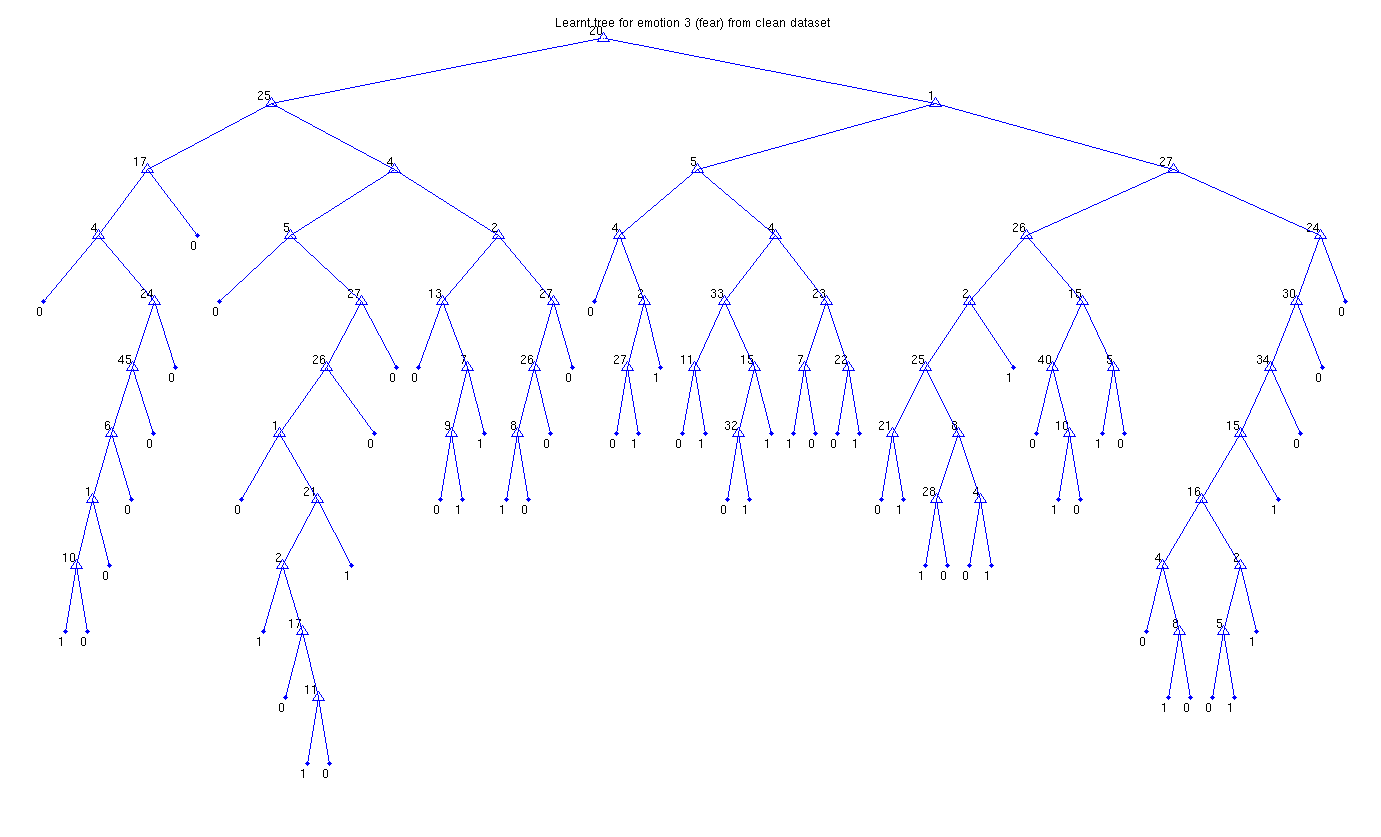
\includegraphics[width=0.75\columnwidth]{FearTree} % Example image
\caption{Trained decsion tree on the clean dataset for emotion 3 (fear)}
\end{figure}

\begin{figure}[!ht]
\center
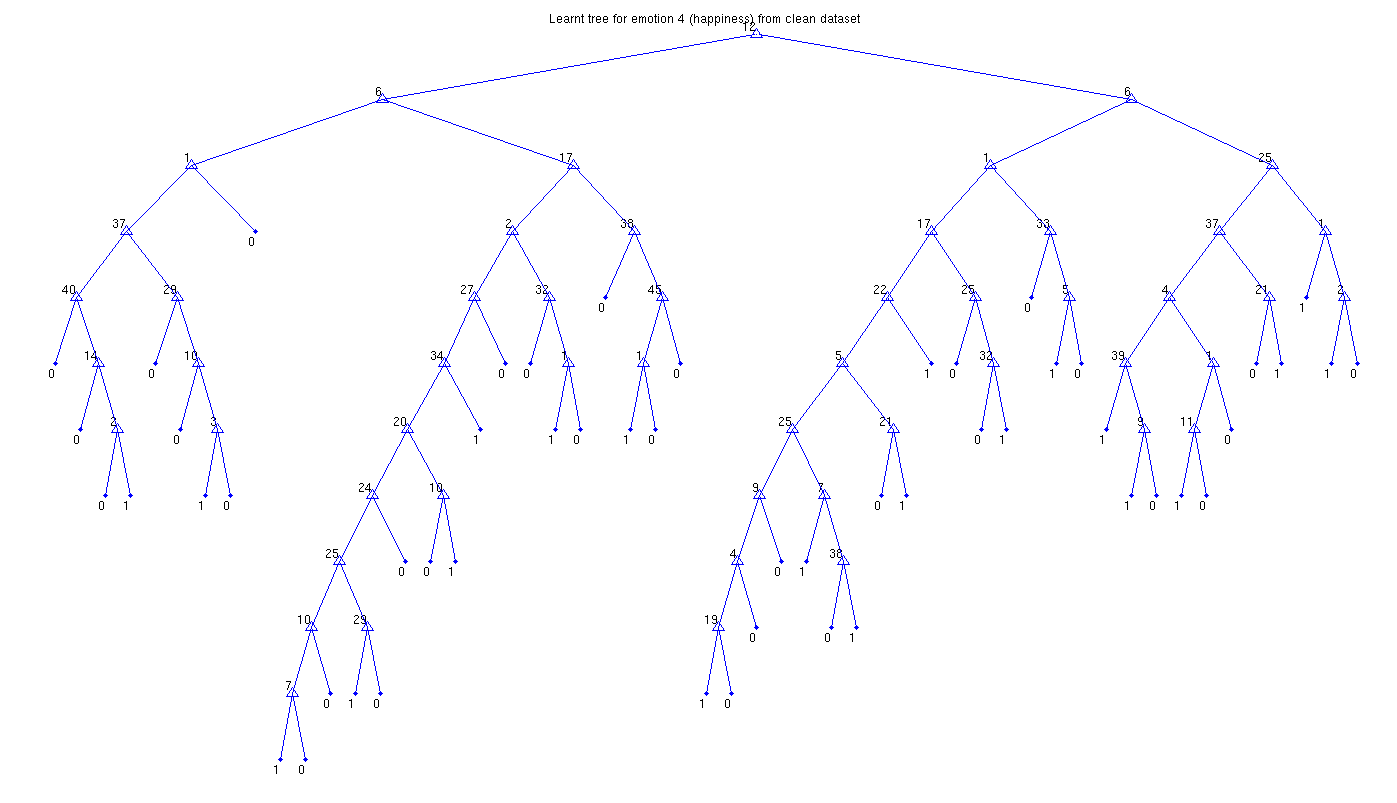
\includegraphics[width=0.75\columnwidth]{HappinessTree} % Example image
\caption{Trained decsion tree on the clean dataset for emotion 4 (happiness)}
\end{figure}

\begin{figure}[!ht]
\center
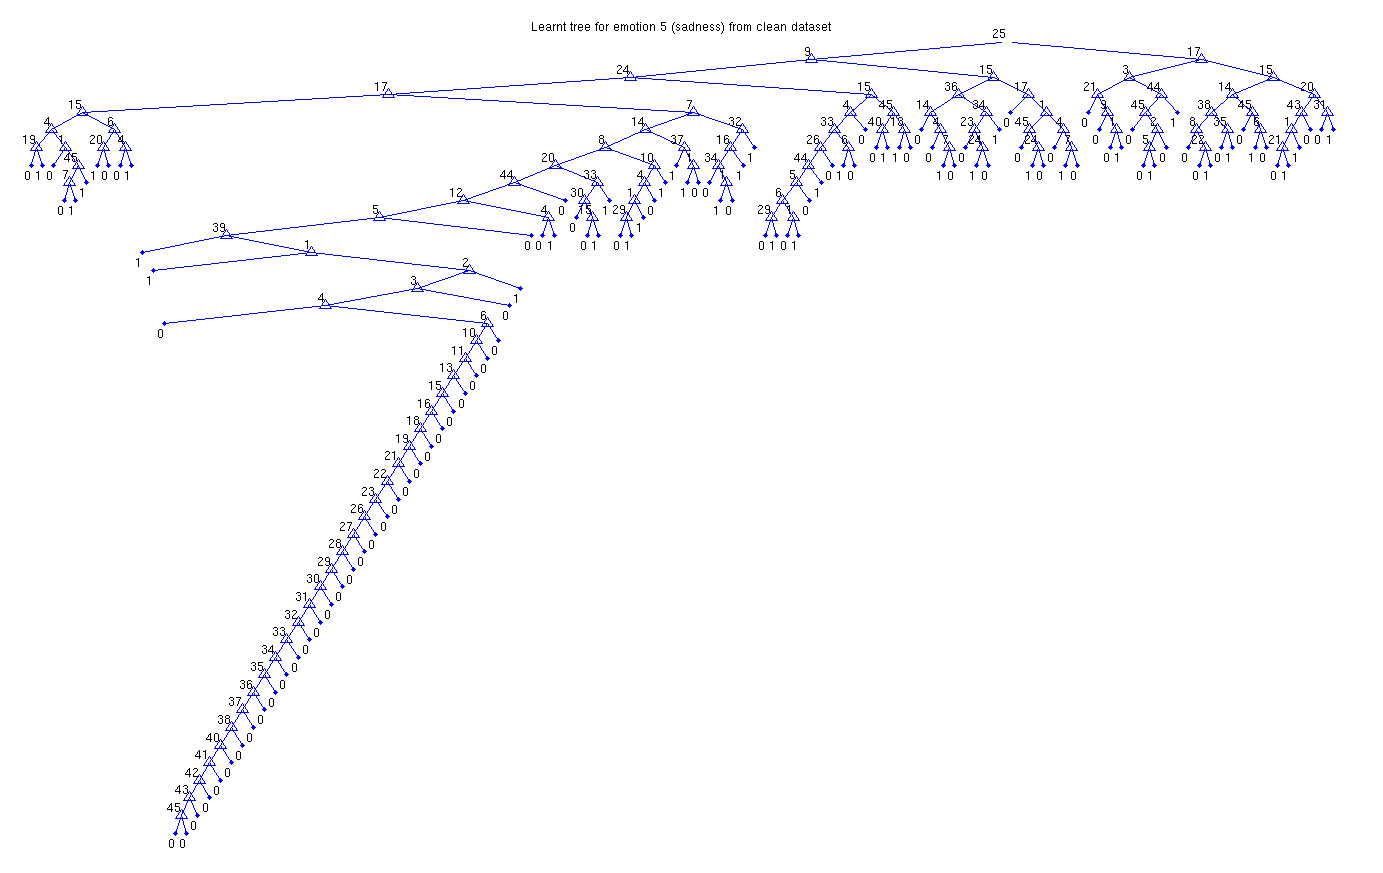
\includegraphics[width=0.75\columnwidth]{SadnessTree} % Example image
\caption{Trained decsion tree on the clean dataset for emotion 5 (sadness)}
\end{figure}

\begin{figure}[!ht]
\center
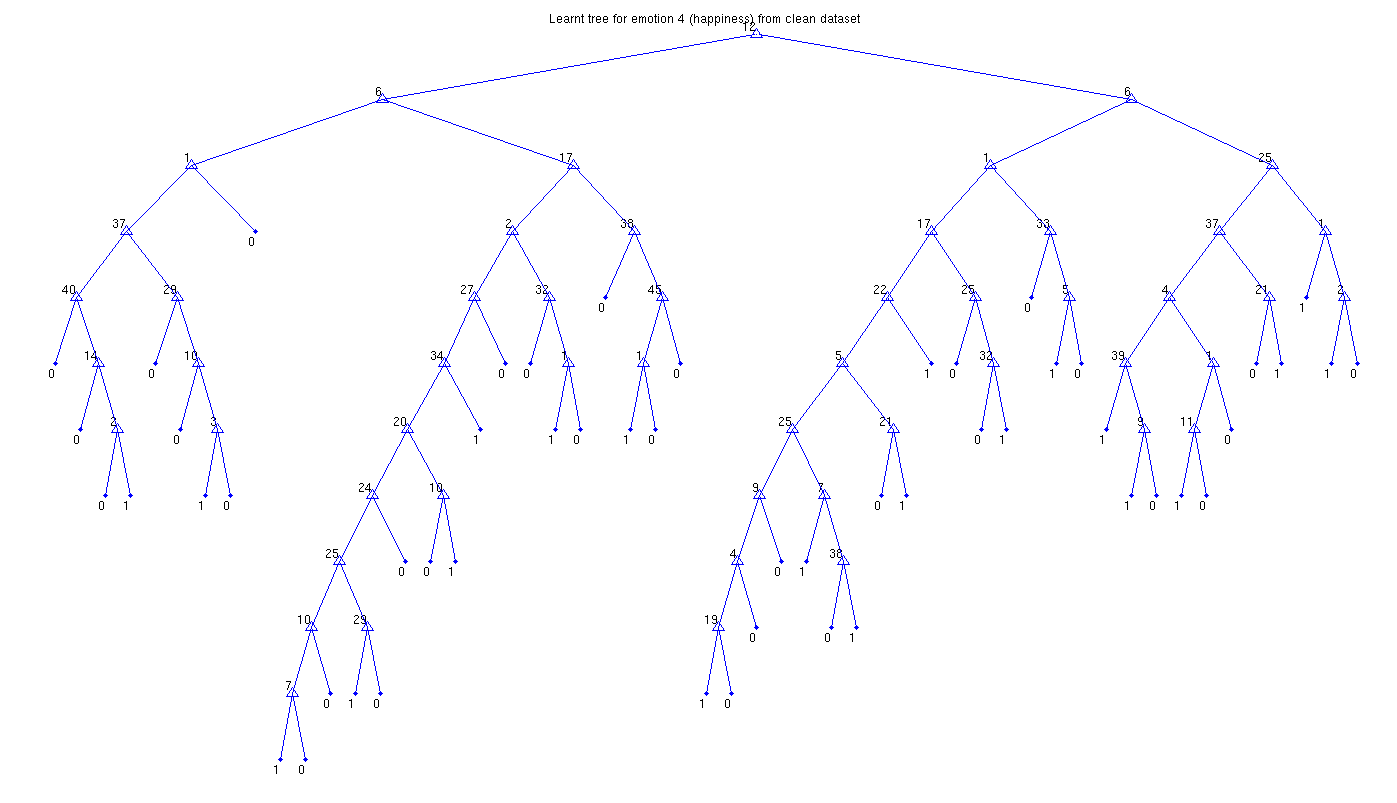
\includegraphics[width=0.75\columnwidth]{HappinessTree} % Example image
\caption{Trained decsion tree on the clean dataset for emotion 6 (surprise)}
\end{figure}

\clearpage

%----------------------------------------------------------------------------------------
%	SECTION 3 - Evaluation
%----------------------------------------------------------------------------------------

\section{Evaluation}

\subsection{Clean dataset}
\subsubsection{Confusion matrix}

\begin{table}[H]
\center
\begin{tabu}{cc|c|c|c|c|c|c|}
\cline{3-8}
& & \multicolumn{6}{ c| }{Predicted class} \\ \cline{3-8}
& & 1 & 2 & 3 & 4 & 5 & 6 \\ \cline{1-2} \tabucline[1.5pt]{3-8}
\multicolumn{1}{ |c| }{\multirow{6}{*}{Actual class} } &
\multicolumn{1}{ |c|[1.5pt] }{1} & \textbf{85} & 15 & 4 & 9 & 17 & 2 \\ \cline{2-8}
\multicolumn{1}{ |c| }{}                        &
\multicolumn{1}{ |c|[1.5pt] }{2} & 17 & \textbf{137} & 5 & 12 & 15 & 12 \\ \cline{2-8}
\multicolumn{1}{ |c|  }{}                        &
\multicolumn{1}{ |c|[1.5pt] }{3} & 8 & 7 & \textbf{80} & 0 & 10 & 14 \\ \cline{2-8}
\multicolumn{1}{ |c|  }{}                        &
\multicolumn{1}{ |c|[1.5pt] }{4} & 4 & 12 & 8 & \textbf{177} & 9 & 6 \\ \cline{2-8}
\multicolumn{1}{ |c|  }{}                        &
\multicolumn{1}{ |c|[1.5pt] }{5} & 15 & 10 & 11 & 11 & \textbf{75} & 10 \\ \cline{2-8}
\multicolumn{1}{ |c|  }{}                        &
\multicolumn{1}{ |c|[1.5pt] }{6} & 3 & 10 & 11 & 6 & 11 & \textbf{166} \\ \cline{1-8}
\end{tabu}
\caption{Confusion Matrix for the \emph{clean} dataset (Strategy 1 - see next section)}
\label{confusionMatrixCleanStrategyOne}
\end{table}

\subsubsection{Recall, precision and $F_1$ measure}

\begin{table}[H]
\center
\begin{tabu}{cc|c|c|c|}
\cline{3-5}
& & Recall & Precision & $F_1$ \\ \cline{1-2} \tabucline[1.5pt]{3-5}
\multicolumn{1}{ |c| }{\multirow{6}{*}{Actual class} } &
\multicolumn{1}{ |c|[1.5pt] }{1} & 64\% & 64\% & 64\% \\ \cline{2-5}
\multicolumn{1}{ |c| }{}                        &
\multicolumn{1}{ |c|[1.5pt] }{2} & 69\% & 72\% & 70\% \\ \cline{2-5}
\multicolumn{1}{ |c|  }{}                        &
\multicolumn{1}{ |c|[1.5pt] }{3} & 67\% & 67\% & 67\% \\ \cline{2-5}
\multicolumn{1}{ |c|  }{}                        &
\multicolumn{1}{ |c|[1.5pt] }{4} & 82\% & 82\% & 82\% \\ \cline{2-5}
\multicolumn{1}{ |c|  }{}                        &
\multicolumn{1}{ |c|[1.5pt] }{5} & 57\% & 55\% & 56\% \\ \cline{2-5}
\multicolumn{1}{ |c|  }{}                        &
\multicolumn{1}{ |c|[1.5pt] }{6} & 80\% & 79\% & 80\% \\ \cline{1-5}
\end{tabu}
\caption{Recall, precision and $F_1$ measure for the \emph{clean} dataset (Strategy 1 - see next section)}
\label{recallPrecisionF1Clean}
\end{table}

\subsubsection{Average classification rate}

\[ C = \frac{720}{1004} = 71.7\% \]

\subsection{Noisy dataset}
\subsubsection{Confusion matrix}

\begin{table}[H]
\center
\begin{tabu}{cc|c|c|c|c|c|c|}
\cline{3-8}
& & \multicolumn{6}{ c| }{Predicted class} \\ \cline{3-8}
& & 1 & 2 & 3 & 4 & 5 & 6 \\ \cline{1-2} \tabucline[1.5pt]{3-8}
\multicolumn{1}{ |c| }{\multirow{6}{*}{Actual class} } &
\multicolumn{1}{ |c|[1.5pt] }{1} & \textbf{25} & 11 & 16 & 5 & 22 & 9 \\ \cline{2-8}
\multicolumn{1}{ |c| }{}                        &
\multicolumn{1}{ |c|[1.5pt] }{2} & 12 & \textbf{127} & 13 & 19 & 8 & 8 \\ \cline{2-8}
\multicolumn{1}{ |c|  }{}                        &
\multicolumn{1}{ |c|[1.5pt] }{3} & 17 & 13 & \textbf{104} & 19 & 14 & 20 \\ \cline{2-8}
\multicolumn{1}{ |c|  }{}                        &
\multicolumn{1}{ |c|[1.5pt] }{4} & 11 & 11 & 13 & \textbf{154} & 6 & 14 \\ \cline{2-8}
\multicolumn{1}{ |c|  }{}                        &
\multicolumn{1}{ |c|[1.5pt] }{5} & 17 & 7 & 7 & 12 & \textbf{56} & 11 \\ \cline{2-8}
\multicolumn{1}{ |c|  }{}                        &
\multicolumn{1}{ |c|[1.5pt] }{6} & 10 & 14 & 21 & 9 & 11 & \textbf{155} \\ \cline{1-8}
\end{tabu}
\caption{Confusion Matrix for the \emph{noisy} dataset (Strategy 1 - see next section)}
\label{confusionMatrixNoisyStrategyOne}
\end{table}

\subsubsection{Recall, precision and $F_1$ measure}

\begin{table}[H]
\center
\begin{tabu}{cc|c|c|c|}
\cline{3-5}
& & Recall & Precision & $F_1$ \\ \cline{1-2} \tabucline[1.5pt]{3-5}
\multicolumn{1}{ |c| }{\multirow{6}{*}{Actual class} } &
\multicolumn{1}{ |c|[1.5pt] }{1} & 28\% & 27\% & 28\% \\ \cline{2-5}
\multicolumn{1}{ |c| }{}                        &
\multicolumn{1}{ |c|[1.5pt] }{2} & 68\% & 69\% & 69\% \\ \cline{2-5}
\multicolumn{1}{ |c|  }{}                        &
\multicolumn{1}{ |c|[1.5pt] }{3} & 56\% & 60\% & 58\% \\ \cline{2-5}
\multicolumn{1}{ |c|  }{}                        &
\multicolumn{1}{ |c|[1.5pt] }{4} & 74\% & 71\% & 72\% \\ \cline{2-5}
\multicolumn{1}{ |c|  }{}                        &
\multicolumn{1}{ |c|[1.5pt] }{5} & 51\% & 48\% & 49\% \\ \cline{2-5}
\multicolumn{1}{ |c|  }{}                        &
\multicolumn{1}{ |c|[1.5pt] }{6} & 70\% & 71\% & 71\% \\ \cline{1-5}
\end{tabu}
\caption{Recall, precision and $F_1$ measure for the \emph{noisy} dataset (Strategy 1 - see next section)}
\label{recallPrecisionF1Noisy}
\end{table}

\subsubsection{Average classification rate}

\[ C = \frac{621}{1004} = 61.9\% \]

\clearpage

%----------------------------------------------------------------------------------------
%	SECTION 4 - Questions
%----------------------------------------------------------------------------------------

\section{Questions}
\subsection{Noisy-Clean Datasets}

\subsection{Ambiguity}
\subsubsection{Description of methods}

We tried three methods for assignment of a single value to examples which have been positively classified by more than one tree:
\begin{enumerate} \itemsep0pt \parskip0pt \parsep0pt
  \item Assign a \emph{random} class from the set of predicted classes
  \item Assign a class which has been returned at a \emph{smallest depth}
  \item Assign a class which has been returned at a \emph{greatest depth}
\end{enumerate}
Advantages of the first method include the fact that it is the simplest and easiest to implement. Additionally, it serves as a nice benchmark for the other methods. It allows to see whether they preform any better than just a simple random assignment. Obviously, the main disadvantage is that the method does not use any clever heuristic in order to classify the examples. Evaluation of Strategy 1 has been presented in the previous section. \smallskip

The intuition behind the second method is that the smaller number of steps a tree needs to take in order to classify an emotion, the more "sure" it should be of the emotion being accurately classified. On the other hand, should that intuition prove to be incorrect, we also wanted to see what would be the performance of an exact opposite algorithm, which is the third method outlined above. Both methods require us to store the depth of the returned solution, in addition to the classification results of the 6 trees (in a $Nx6$ matrix). This increases the memory requirements in comparison to Strategy 1.

\subsubsection{Evaluation of Strategy 2}



\subsubsection{Evaluation of Strategy 3}



\subsubsection{Comparison of methods}



\subsection{Pruning}

\clearpage

%----------------------------------------------------------------------------------------
%	SECTION 5 - Code Flowchart
%----------------------------------------------------------------------------------------

\section{Code Flowchart}

\clearpage

%----------------------------------------------------------------------------------------

\end{document}